%%%%%%%%%%%%%%%%%%%%%%%%%%%%%%%%%%%%%%%%%
% Short Sectioned Assignment
% LaTeX Template
% Version 1.0 (5/5/12)
%
% This template has been downloaded from:
% http://www.LaTeXTemplates.com
%
% Original author:
% Frits Wenneker (http://www.howtotex.com)
%
% License:
% CC BY-NC-SA 3.0 (http://creativecommons.org/licenses/by-nc-sa/3.0/)
%
%%%%%%%%%%%%%%%%%%%%%%%%%%%%%%%%%%%%%%%%%

%----------------------------------------------------------------------------------------
%	PACKAGES AND OTHER DOCUMENT CONFIGURATIONS
%----------------------------------------------------------------------------------------

\documentclass[paper=a4, fontsize=11pt]{scrartcl} % A4 paper and 11pt font size

\usepackage{graphicx}
\usepackage[T1]{fontenc} % Use 8-bit encoding that has 256 glyphs
\usepackage{fourier} % Use the Adobe Utopia font for the document - comment this line to return to the LaTeX default
\usepackage[english]{babel} % English language/hyphenation
\usepackage{amsmath,amsfonts,amsthm} % Math packages

\usepackage{lipsum} % Used for inserting dummy 'Lorem ipsum' text into the template
\usepackage{algorithm}
\usepackage{algpseudocode}
\usepackage{sectsty} % Allows customizing section commands
\allsectionsfont{\scshape} % Make all sections centered, the default font and small caps

\usepackage{algorithm,algpseudocode}% http://ctan.org/pkg/{algorithms,algorithmx}
\algnewcommand{\Inputs}[1]{%
  \State \textbf{Inputs:}
  \Statex \hspace*{\algorithmicindent}\parbox[t]{.8\linewidth}{\raggedright #1}
}
\algnewcommand{\Initialize}[1]{%
  \State \textbf{Initialize:}
  \Statex \hspace*{\algorithmicindent}\parbox[t]{.8\linewidth}{\raggedright #1}
}

\usepackage{fancyhdr} % Custom headers and footers
\pagestyle{fancyplain} % Makes all pages in the document conform to the custom headers and footers
\fancyhead{} % No page header - if you want one, create it in the same way as the footers below
\fancyfoot[L]{} % Empty left footer
\fancyfoot[C]{} % Empty center footer
\fancyfoot[R]{\thepage} % Page numbering for right footer
\renewcommand{\headrulewidth}{0pt} % Remove header underlines
\renewcommand{\footrulewidth}{0pt} % Remove footer underlines
\setlength{\headheight}{13.6pt} % Customize the height of the header

\numberwithin{equation}{section} % Number equations within sections (i.e. 1.1, 1.2, 2.1, 2.2 instead of 1, 2, 3, 4)
\numberwithin{figure}{section} % Number figures within sections (i.e. 1.1, 1.2, 2.1, 2.2 instead of 1, 2, 3, 4)
\numberwithin{table}{section} % Number tables within sections (i.e. 1.1, 1.2, 2.1, 2.2 instead of 1, 2, 3, 4)

\setlength\parindent{0pt} % Removes all indentation from paragraphs - comment this line for an assignment with lots of text

%----------------------------------------------------------------------------------------
%	TITLE SECTION
%----------------------------------------------------------------------------------------

\newcommand{\horrule}[1]{\rule{\linewidth}{#1}} % Create horizontal rule command with 1 argument of height

\title{	
\normalfont \normalsize
\textsc{Rice University, Department of Computer Science} \\ [25pt] % Your university, school and/or department name(s)
\horrule{0.5pt} \\[0.4cm] % Thin top horizontal rule
\huge Assignment 4, COMP 540 \\ % The assignment title
\horrule{2pt} \\[0.5cm] % Thick bottom horizontal rule
}

\author{Chen Zeng(cz39), Zhihui Xie(zx18)} % Your name

\date{\normalsize\today} % Today's date or a custom date

\begin{document}

\maketitle % Print the title

\section{Intuitions about support vector machines}
\paragraph{\textbf{Answer1}}

%If we train a SVM classifier by providing the patterns and associated labels as input, the result of this supervised learning will be a decision boundary (a straight line in the linear case) separating the two classes. It is obvious that there are many lines, which would correctly separate the two classes.  The SVMs strive for an optimal separating line, which should be as far as possible away from the points in both classes. 
%\\ 
The margin is the distance of the separation line to the closest points of each class. Intuitively, bigger margin makes it to be more robust to noise and it can give a safer decision boundary. It means a little error in measurement of the input won't lead to misclassification. 
\\ Thus, intuitively, a bigger margin will result in a model that will generalize better, or perform better in practice.
% \\ Ref: http://www.brainvoyager.com/bvqx/doc/UsersGuide/MVPA/SupportVectorMachinesSVMs.html

\paragraph{\textbf{Answer2}}
%No, it won't. The decision boundary is only determined by support vectors. According to the instruction in sparse\_kernels.pdf, we can find the conclusion that moving non-support vector does not change decision boundary.
%\\ Here is the detailed reason. To classify a new $x$
%\begin{equation*}
%h_{\theta }\left ( x \right )=Sign\left ( \theta ^{T}x+\theta _{0} \right )=Sign\left ( \sum_{i=1}^{m}\alpha ^{\left ( i \right )}y ^{\left ( i \right )} x ^{\left ( i \right )T}x+\theta _{0}\right )
%\end{equation*}
%Since $\alpha ^{\left ( i \right )}>0$ only for support vector, we only need to maintain support vector once we calculate $\theta_{0}$. Therefore, moving points which are not support vectors further away from the decision boundary won't effect the SVM?s hinge loss.
No, it won't. The hinge loss function is defined as $J\left ( \theta ,\theta _{0} \right )=C\sum_{i=1}^{m}max\left ( 0,1-y^{\left ( i \right )}h_{\theta }\left ( x^{\left ( i \right )} \right ) \right )$. As for points that are not support vectors, the second term of max function is negative and moving them to be further away from the decision boundary will make it to be more negative. Therefore, no matter how you remove them, the max function will return 0. It proves that the loss function is entirely determined by the support vectors.

\section{Fitting an SVM classifier by hand}

\paragraph{\textbf{Answer1}}
According to the feature vector $\phi \left ( x \right )=\left ( 1,\sqrt{x},x^{2} \right )$, we can map the point $\left ( x^{\left ( 1 \right )},y^{\left ( 1 \right )} \right )$ and $\left ( x^{\left ( 2 \right )},y^{\left ( 2 \right )} \right )$ which are $\left( 0,-1 \right )$ and $\left( 2,+1 \right )$ to $\left( \phi \left ( x^{\left ( 1 \right )} \right ),y^{\left ( 1 \right )} \right )$ and $\left( \phi \left ( x^{\left ( 2 \right )} \right ),y^{\left ( 2 \right )} \right )$ which are $\left ( \left ( 1,0,0 \right ),-1 \right )$ and $\left ( \left (1,2,2 \right ),+1 \right )$.
\\ Let's suppose that the line cross these two points in three-dimension has the quation of $ax+by+cz=d$. Because $\phi \left ( x^{\left ( 1 \right )} \right )=\left ( 1,0,0 \right )$ and $\phi \left ( x^{\left ( 2 \right )} \right )=\left ( 1,2,2 \right )$ are on the line, we can get:
\begin{equation*}
\left\{\begin{matrix}
a=d\\ 
a+2b+2c=d
\end{matrix}\right.\Rightarrow 
\left\{\begin{matrix}
a=d\\ 
b+c=0
\end{matrix}\right.
\end{equation*}
Therefore, the line cross these two points in three-dimension meets the following equation:
\begin{equation*}
\left\{\begin{matrix}
x=1\\ 
y=z
\end{matrix}\right.
\end{equation*}
Because the optima vector $\theta$ should be on this line, this question is just to find a vector which is parallel to the above line. For example, the following scaled vector can meet with this requirement:
\begin{equation*}
\theta^{'} = \left(0, \frac{\sqrt{2}}{2}, \frac{\sqrt{2}}{2}\right)^{T}
\end{equation*}

\paragraph{\textbf{Answer2}}
The decision boundary is vertical to $\theta$. Because the value of margin is the distance from each support vector to the decision boundary, which is half the distance between two points. And these two points are symmetry to the decision boundary. Thus, the value of margin should be the distance between $\phi \left ( x^{\left ( 1 \right )} \right )=\left ( 1,0,0 \right )$ and $\phi \left ( x^{\left ( 2 \right )} \right )=\left ( 1,2,2 \right )$. Here we can calculate it:
\begin{equation*}
margin=\frac{1}{2}dis\left ( \phi \left ( x^{\left ( 1 \right )} \right ), \phi \left ( x^{\left ( 2 \right )} \right ) \right )=\frac{1}{2}dis\left ( \left ( 1,0,0 \right ),\left ( 1,2,2 \right ) \right )=\frac{1}{2}\sqrt{\left ( 1-1 \right )^{2}+\left ( 0-2 \right )^{2}+\left ( 0-2 \right )^{2}}=\sqrt{2}
\end{equation*}
Therefore, the value of margin is $\sqrt{2}$.

\paragraph{\textbf{Answer3}}
%According to the statement, we need to solve the following constrained quadratic optimization problem:
%\begin{align*}
%&min \frac{1}{2}\left \| \theta  \right \|^{2} 
%\\ s.t &
%\\ &y^{\left ( 1 \right )}\left ( \theta ^{T}\phi \left ( x^{\left ( 1 \right )} \right )+\theta _{0} \right )\geq 1
%\\ &y^{\left ( 2 \right )}\left ( \theta ^{T}\phi \left ( x^{\left ( 2 \right )} \right )+\theta _{0} \right )\geq 1
%\end{align*}
%We can solve the QP using the method of Lagrange multiplier:
%\begin{equation*}
%L\left ( \theta ,\theta _{0},\alpha  \right )=\frac{1}{2}\left \| \theta  \right \|^{2}-\sum_{i=1}^{m}\alpha ^{\left ( i \right )}\left [ \left ( \theta ^{T}x^{\left ( i \right )}+\theta _{0} \right )y^{\left ( i \right )}-1 \right ]
%\end{equation*}
%Let's take the value of $\phi \left ( x^{\left ( 1 \right )} \right )=\left ( 1,0,0 \right )$ and $\phi \left ( x^{\left ( 2 \right )} \right )=\left ( 1,2,2 \right )$ into the above equation, we can get the following equation:
%\begin{equation*}
%L\left ( \theta _{0},\theta _{1},\theta _{2},\theta _{3},\alpha ^{\left ( 1 \right )},\alpha ^{\left ( 2 \right )} \right )=\frac{1}{2}\left ( \theta _{1}^2+\theta _{2}^2+\theta _{3}^2 \right )-\alpha ^{\left ( 1 \right )}\left [- \left ( \theta _{1}+\theta _{0} \right )-1 \right ]-\alpha ^{\left ( 2 \right )}\left [ \left ( \theta _{1}+2\theta _{2}+2\theta _{3}+\theta _{0} \right )-1 \right ]
%\end{equation*}
%Take the gradient of above equation with the following parameters $\theta _{0},\theta _{1},\theta _{2},\theta _{3},\alpha ^{\left ( 1 \right )},\alpha ^{\left ( 2 \right )}$ and make it equal to be 0, we can get the following equations:
%\begin{equation*}
%\frac{\partial L}{\partial \theta _{0}}=\alpha ^{\left ( 1 \right )}-\alpha ^{\left ( 2 \right )}=0
%\end{equation*}
%\begin{equation*}
%\frac{\partial L}{\partial \theta _{1}}=\theta _{1}+\alpha ^{\left ( 1 \right )}-\alpha ^{\left ( 2 \right )}=0
%\end{equation*}
%\begin{equation*}
%\frac{\partial L}{\partial \theta _{2}}=\theta _{2}-2\alpha ^{\left ( 2 \right )}=0
%\end{equation*}
%\begin{equation*}
%\frac{\partial L}{\partial \theta _{3}}=\theta _{3}-2\alpha ^{\left ( 2 \right )}=0
%\end{equation*}
%\begin{equation*}
%\frac{\partial L}{\partial \alpha ^{\left ( 1 \right )}}=\theta _{1}+\theta _{0}+1=0
%\end{equation*}
%\begin{equation*}
%\frac{\partial L}{\partial \alpha ^{\left ( 2 \right )}}=-\left ( \left ( \theta _{1}+2\theta _{2}+2\theta _{3}+\theta _{0} \right )-1 \right ) =0
%\end{equation*}
%We can solve them with the following answers:
%\begin{equation*}
%\theta _{0}=-1, \theta _{1}=0, \theta _{2}=\theta _{3}=\frac{1}{2},\alpha ^{\left ( 1 \right )}=\alpha ^{\left ( 2 \right )}=\frac{1}{4}
%\end{equation*}
%Thus, we've solved out the $\theta$ as:
%\begin{equation*}
%\theta =\left ( 0,\frac{1}{2},\frac{1}{2} \right )
%\end{equation*}
%Therefore, the value of margin is equal to:
%\begin{equation*}
%\frac{1}{\left \| \theta  \right \|}=\frac{1}{\left \| \left ( 0, \frac{1}{2}, \frac{1}{2} \right ) \right \|}=\sqrt{2}
%\end{equation*}
From the statement of this question, we have:
\begin{align*}
margin=\frac{1}{\left \| \theta  \right \|}=\sqrt{2}
\end{align*}
Therefore, we can solve out the value of $\left \| \theta  \right \|$ as below:
\begin{align*}
\left \| \theta  \right \|=\frac{\sqrt{2}}{2}
\end{align*}
As we've got that vector $\theta$ is parallel to the vector $\theta^{'} = \left(0, \frac{\sqrt{2}}{2}, \frac{\sqrt{2}}{2}\right)^{T}$ in answer 1, we can set vector $\theta$ as below:
\begin{align*}
\theta = \left(0, \frac{\sqrt{2}}{2}t, \frac{\sqrt{2}}{2}t\right)^{T}
\end{align*}
Here $t$ is to be solved, and we can get:
\begin{align*}
\left \| \theta \right \| = \left \| \left(0, \frac{\sqrt{2}}{2}t, \frac{\sqrt{2}}{2}t\right)^{T} \right \|=\sqrt{0^{2}+\left ( \frac{\sqrt{2}}{2}t \right )^{2}+\left ( \frac{\sqrt{2}}{2}t \right )^{2}}=\left | t \right |
\end{align*}
At the same time, we've got:
\begin{align*}
\left \| \theta  \right \|=\frac{\sqrt{2}}{2}
\end{align*}
Therefore, we can get the value of $t$ as below:
\begin{align*}
t=\pm \frac{\sqrt{2}}{2} 
\end{align*}
It means there are two possible for vector $\theta$:
\begin{align*}
\theta =\pm \left ( 0, \frac{1}{2}, \frac{1}{2} \right ) ^{T}
\end{align*}
However, the following requirements need to be fulfilled:
\begin{align*}
&y^{\left ( 1 \right )}\left ( \theta ^{T}\phi \left ( x^{\left ( 1 \right )} \right )+\theta _{0} \right )\geq 1
\\ &y^{\left ( 2 \right )}\left ( \theta ^{T}\phi \left ( x^{\left ( 2 \right )} \right )+\theta _{0} \right )\geq 1
\end{align*}
Let's take the value of $y^{\left ( 1 \right )}=-1$, $y^{\left ( 2 \right )}=1$, $\phi \left ( x^{\left ( 1 \right )} \right )=\left ( 1,0,0 \right )$, and $\phi \left ( x^{\left ( 2 \right )} \right )=\left ( 1,2,2 \right )$ into it, we can get the following restrictions:
\begin{align*}
&-\left ( \theta _{0}+\theta _{1} \right )\geq 1
\\ &\theta _{0}+\theta _{1}+2\theta _{2}+2\theta _{3}\geq 1
\end{align*}
Therefore, we can get the transformation:
\begin{align*}
\theta _{2}+\theta _{3}\geq \frac{1}{2}\left ( -\left (  \theta _{0}+\theta _{1}\right ) +1\right )\geq \frac{1}{2}\left ( 1+1 \right )=1
\end{align*}
Because the final result must meet the above restriction which is $\theta _{2}+\theta _{3}\geq1$, here we have only one positive final result of $\theta$ as below:
\begin{align*}
\theta =\left ( 0, \frac{1}{2}, \frac{1}{2} \right ) ^{T}
\end{align*}

\paragraph{\textbf{Answer4}}
%From the answer of last problem, we've got the value of $\theta_{0}$ as
%\begin{equation*}
%\theta_{0}=-1
%\end{equation*}
Let's take the value of $y^{\left ( 1 \right )}=-1$ and $y^{\left ( 2 \right )}=1$ into following equations:
\begin{equation*}
y^{\left ( 1 \right )}\left ( \theta ^{T}\phi \left ( x^{\left ( 1 \right )} \right )+\theta _{0} \right )=1
\end{equation*}
\begin{equation*}
y^{\left ( 2 \right )}\left ( \theta ^{T}\phi \left ( x^{\left ( 2 \right )} \right )+\theta _{0} \right )=1
\end{equation*}
We can get the following equations:
\begin{equation*}
\theta ^{T}\phi \left ( x^{\left ( 1 \right )} \right )+\theta _{0} =-1
\end{equation*}
\begin{equation*}
\theta ^{T}\phi \left ( x^{\left ( 2 \right )} \right )+\theta _{0} =1
\end{equation*}
From the value we get in the above solutions, we have:
\begin{equation*}
\theta ^{T}\phi \left ( x^{\left ( 1 \right )} \right )=\left ( 0, \frac{1}{2}, \frac{1}{2} \right ) ^{T}\left ( 1,0,0 \right )=0
\end{equation*}
\begin{equation*}
\theta ^{T}\phi \left ( x^{\left ( 2 \right )} \right )=\left ( 0, \frac{1}{2}, \frac{1}{2} \right ) ^{T}\left ( 1,2,2 \right )=2
\end{equation*}
Therefore, we can get:
\begin{equation*}
0+\theta _{0} =-1
\end{equation*}
\begin{equation*}
2+\theta _{0} =1
\end{equation*}
Thus, the final result is that:
\begin{equation*}
\theta _{0} =-1
\end{equation*}

\paragraph{\textbf{Answer5}}
Let the following $\phi \left ( x \right )$ be equal to 0:
\begin{align*}
%h_{\theta }\left ( x \right )=&Sign\left ( \theta ^{T}x+\theta _{0} \right )
%\\ =&Sign\left ( \sum_{i=1}^{m}\alpha ^{\left ( i \right )}y ^{\left ( i \right )} x ^{\left ( i \right )T}x+\theta _{0}\right )
%\\ =&Sign\left ( -\frac{1}{4}\left [ 1,0,0 \right ]x+\frac{1}{4}\left [ 1,2,2 \right ]x-1 \right )
%\\=&Sign\left ( \frac{1}{4}\left [ 0,2,2 \right ]x-1 \right )
\phi \left ( x \right )=&\theta ^{T}x+\theta _{0}=\left ( 0,\frac{1}{2},\frac{1}{2} \right )\left ( 1,\sqrt{2}x,x^{2} \right )-1
\\=&\frac{1}{2}x^{2}+\frac{\sqrt{2}}{2}x-1
\\=&0
\end{align*}
Here we can get the equation for the decision boundary in terms of $\theta, \theta_{0}, x$:
\begin{align*}
x^{2}+\sqrt{2}x-2=0
\end{align*}

\section{Support vector machines for binary classification}
\paragraph{\textbf{Answer3.1B}}
Figure \ref{fig:decision_boundary} shows the decision boundary for C = 100. It shows as below.
\begin{figure}[H]
 	\centering
 	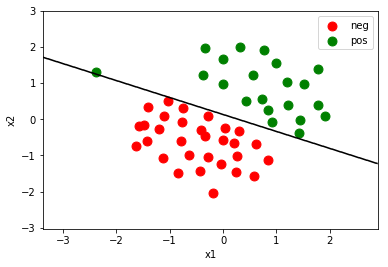
\includegraphics[scale=0.6]{./../output_7_1.png}
 	\caption{decision boundary for C = 100}
 	\label{fig:decision_boundary}
 \end{figure}

\paragraph{\textbf{Answer3.3}}
As for this task, I tried two models: one is Linear Model, and another one is Gaussian Kernel. As for Linear Model, I tried 8 models where C = 0.01, 0.03, 0.1, 0.3, 1, 3, 10, 30.
As for Gaussian Kernel, I tried 8*8=64 models where C = 0.01, 0.03, 0.1, 0.3, 1, 3, 10, 30 and sigma = 0.01 ,0.03, 0.1, 0.3, 1, 3, 10, 30. I trained each of them for 2000 times iterations and test them on dataset. Here are the results:
\begin{verbatim}
1. Using Linear Model:
While C = 0.01 , accuracy on validation data = 0.68625
While C = 0.03 , accuracy on validation data = 0.68625
While C = 0.1 , accuracy on validation data = 0.68625
While C = 0.3 , accuracy on validation data = 0.68625
While C = 1 , accuracy on validation data = 0.69625
While C = 3 , accuracy on validation data = 0.89
While C = 10 , accuracy on validation data = 0.965
While C = 30 , accuracy on validation data = 0.97375
The best case: best_C = 30 , best_accuracy on training data = 0.97375
Accuracy on training data =  0.9709375
Accuracy on test data =  0.973
\end{verbatim}
\begin{verbatim}
2. Using Gaussian Kernel:
While sigma = 0.01 , C = 0.01 , accuracy on validation data = 0.77625
While sigma = 0.01 , C = 0.03 , accuracy on validation data = 0.77625
While sigma = 0.01 , C = 0.1 , accuracy on validation data = 0.77625
While sigma = 0.01 , C = 0.3 , accuracy on validation data = 0.77625
While sigma = 0.01 , C = 1 , accuracy on validation data = 0.77625
While sigma = 0.01 , C = 3 , accuracy on validation data = 0.78125
While sigma = 0.01 , C = 10 , accuracy on validation data = 0.78125
While sigma = 0.01 , C = 30 , accuracy on validation data = 0.78125
While sigma = 0.03 , C = 0.01 , accuracy on validation data = 0.77625
While sigma = 0.03 , C = 0.03 , accuracy on validation data = 0.77625
While sigma = 0.03 , C = 0.1 , accuracy on validation data = 0.77625
While sigma = 0.03 , C = 0.3 , accuracy on validation data = 0.77625
While sigma = 0.03 , C = 1 , accuracy on validation data = 0.77625
While sigma = 0.03 , C = 3 , accuracy on validation data = 0.78125
While sigma = 0.03 , C = 10 , accuracy on validation data = 0.78125
While sigma = 0.03 , C = 30 , accuracy on validation data = 0.78125
While sigma = 0.1 , C = 0.01 , accuracy on validation data = 0.78375
While sigma = 0.1 , C = 0.03 , accuracy on validation data = 0.78375
While sigma = 0.1 , C = 0.1 , accuracy on validation data = 0.78375
While sigma = 0.1 , C = 0.3 , accuracy on validation data = 0.78375
While sigma = 0.1 , C = 1 , accuracy on validation data = 0.78375
While sigma = 0.1 , C = 3 , accuracy on validation data = 0.78375
While sigma = 0.1 , C = 10 , accuracy on validation data = 0.79125
While sigma = 0.1 , C = 30 , accuracy on validation data = 0.79125
While sigma = 0.3 , C = 0.01 , accuracy on validation data = 0.7925
While sigma = 0.3 , C = 0.03 , accuracy on validation data = 0.7925
While sigma = 0.3 , C = 0.1 , accuracy on validation data = 0.7925
While sigma = 0.3 , C = 0.3 , accuracy on validation data = 0.7925
While sigma = 0.3 , C = 1 , accuracy on validation data = 0.7925
While sigma = 0.3 , C = 3 , accuracy on validation data = 0.7925
While sigma = 0.3 , C = 10 , accuracy on validation data = 0.8
While sigma = 0.3 , C = 30 , accuracy on validation data = 0.8
While sigma = 1 , C = 0.01 , accuracy on validation data = 0.78875
While sigma = 1 , C = 0.03 , accuracy on validation data = 0.78875
While sigma = 1 , C = 0.1 , accuracy on validation data = 0.78875
While sigma = 1 , C = 0.3 , accuracy on validation data = 0.78875
While sigma = 1 , C = 1 , accuracy on validation data = 0.78875
While sigma = 1 , C = 3 , accuracy on validation data = 0.785
While sigma = 1 , C = 10 , accuracy on validation data = 0.785
While sigma = 1 , C = 30 , accuracy on validation data = 0.7875
While sigma = 3 , C = 0.01 , accuracy on validation data = 0.79
While sigma = 3 , C = 0.03 , accuracy on validation data = 0.79
While sigma = 3 , C = 0.1 , accuracy on validation data = 0.79
While sigma = 3 , C = 0.3 , accuracy on validation data = 0.79
While sigma = 3 , C = 1 , accuracy on validation data = 0.77625
While sigma = 3 , C = 3 , accuracy on validation data = 0.765
While sigma = 3 , C = 10 , accuracy on validation data = 0.755
While sigma = 3 , C = 30 , accuracy on validation data = 0.7475
While sigma = 10 , C = 0.01 , accuracy on validation data = 0.79375
While sigma = 10 , C = 0.03 , accuracy on validation data = 0.79375
While sigma = 10 , C = 0.1 , accuracy on validation data = 0.79375
While sigma = 10 , C = 0.3 , accuracy on validation data = 0.78875
While sigma = 10 , C = 1 , accuracy on validation data = 0.79
While sigma = 10 , C = 3 , accuracy on validation data = 0.7925
While sigma = 10 , C = 10 , accuracy on validation data = 0.78625
While sigma = 10 , C = 30 , accuracy on validation data = 0.77
While sigma = 30 , C = 0.01 , accuracy on validation data = 0.83
While sigma = 30 , C = 0.03 , accuracy on validation data = 0.83
While sigma = 30 , C = 0.1 , accuracy on validation data = 0.83
While sigma = 30 , C = 0.3 , accuracy on validation data = 0.8275
While sigma = 30 , C = 1 , accuracy on validation data = 0.8275
While sigma = 30 , C = 3 , accuracy on validation data = 0.83
While sigma = 30 , C = 10 , accuracy on validation data = 0.825
While sigma = 30 , C = 30 , accuracy on validation data = 0.8175
The best case: best_sigma = 30 , best_C = 0.01 , best_accuracy on training data = 0.83
Accuracy on training data =  0.9878125
Accuracy on test data =  0.831
\end{verbatim}
To conclude, we find the best model is to use Linear Model with C = 30. Therefore, I use this model to train the final model to get spam words with 20000 times iterations. And here are the result of testing accuracy and Top 15 spam and ham words:
\begin{verbatim}
Accuracy on training data =  0.993125
Accuracy on test data =  0.988

Top 15 words predicted to be spam are:
click
remov
our
nbsp
basenumb
free
your
will
guarante
pleas
you
here
most
visit
offer

Top 15 words predicted to be ham are:
wrote
date
the
httpaddr
url
spamassassin
re
numbertnumb
it
thei
user
list
my
author
prefer
\end{verbatim}


\section{Support vector machines for multi-class classification}
\paragraph{\textbf{Answer 4A}}
The zero loss function is not differentiable. Thus, the numerical cannot successfully check. This can be caused by the discrepancy stated in the question.
\\ However, it's not a reason for concern. Because this rarely happens and we usually have a large amount of data.
\paragraph{\textbf{Answer 4D}}
The best case is: 
\begin{verbatim}
lr 5.000000e-08 reg 5.000000e+04 train accuracy: 0.371776 val accuracy: 0.382000
\end{verbatim}
More detailed results can be found in the notebook submitted.

\paragraph{\textbf{Answer 4E}}
Firstly, let's compare the run time and performance of softmax and multi-class SVM regression:
\\ The run time of multi-class SVM regression is shorter than softmax.
\\ The total prediction accuracy of softmax regression in the last assignment:
\begin{verbatim}
softmax on raw pixels final test set accuracy: 0.398700
\end{verbatim}
The total prediction accuracy of multi-class SVM in this assignment:
\begin{verbatim}
linear SVM on raw pixels final test set accuracy: 0.368700
\end{verbatim}
Also, we can compare the prediction accuracy on different classes as below:
\begin{table}[H]
	\centering
	%\caption{Comparing Classifier Accuracy of OVA and Softmax Regression}
	\label{comparing_table}
	\begin{tabular}{lllllllllll}
	Classes            & plane & car   & bird  & cat   & deer  & dog   & frog  & horse & ship  & truck \\
	Softmax & 0.465 & 0.486 & 0.242 & 0.266 & 0.299 & 0.347 & 0.502 & 0.425 & 0.621 & 0.459 \\
	SVM                & 0.407 & 0.469 & 0.297 & 0.298 & 0.336 & 0.343 & 0.315 & 0.487 & 0.381 & 0.393 
	\end{tabular}
\end{table}
From the above comparing on prediction accuracy, we can find on CIFAR-10 task, softmax regression can achieve slightly higher performance. In general, their performance don't different too much.
\\
\\ Secondly, let's compare the visualizations of the $\theta$ parameters. \ref{fig:softmax_theta} is the figure showing visualizations of $\theta$ parameters in softmax regression and \ref{fig:SVM_theta} is the figure showing visualizations of $\theta$ parameters in multi-class SVM. From my perspective of view, we cannot clearly figure out which result of the training model is better from viewing the visualizations of $\theta$ parameters. They seems to be very close.
\begin{figure}[H]
 	\centering
 	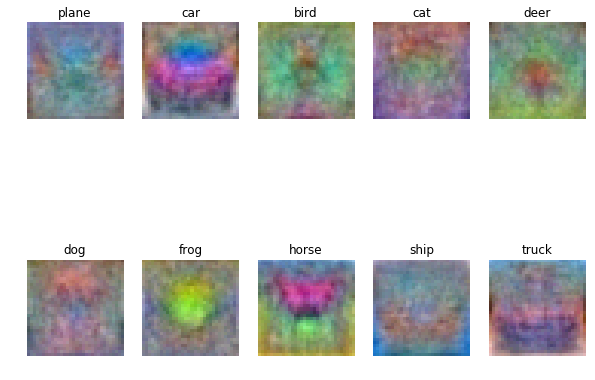
\includegraphics[scale=0.36]{./../softmax_theta}
 	\caption{visualizations of theta parameters in softmax regression}
 	\label{fig:softmax_theta}
\end{figure}
\begin{figure}[H]
 	\centering
 	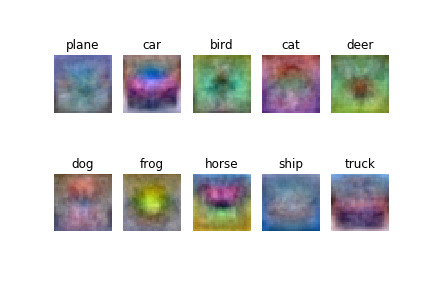
\includegraphics[scale=0.6]{./../multiclass_svm_theta.png}
 	\caption{visualizations of theta parameters in multi-class SVM}
 	\label{fig:SVM_theta}
\end{figure}

Finally, to compare their parameters selection process, we can find both of them need to consider the parameter $learning\_rate$ and $regularization\_strength$. And sometimes both of them need to be considered with $batch\_size$ and $iteration$ in the training process. Therefore, the parameters need to be considered in sofatmax regression and multi-class SVM are same and their parameters selection process are very similar.

\end{document}

